\section{1174096 - Nico Ekklesia Sembiring}
\subsection{Soal Teori}
\begin{enumerate}

	\item Jelaskan kenapa file suara harus di lakukan MFCC.
	\hfill\break
	Karena MFCC dibutuhkan untuk mengidentifikasi jenis suara. Karena perlunya pengambilan ciri dari suara yang didapat seperti sinyal suara, frekuensi dan gelombang suara untuk dapat diubah menjadi beberapa input lain (Konversi). Karena perlunya komputer untuk mendapat inputan tertentu, maka metode MFCC diperlukan untuk mengkonversi menjadi sesuatu yang dibutuhkan. 
	
    \begin{figure}[H]
	\centering
		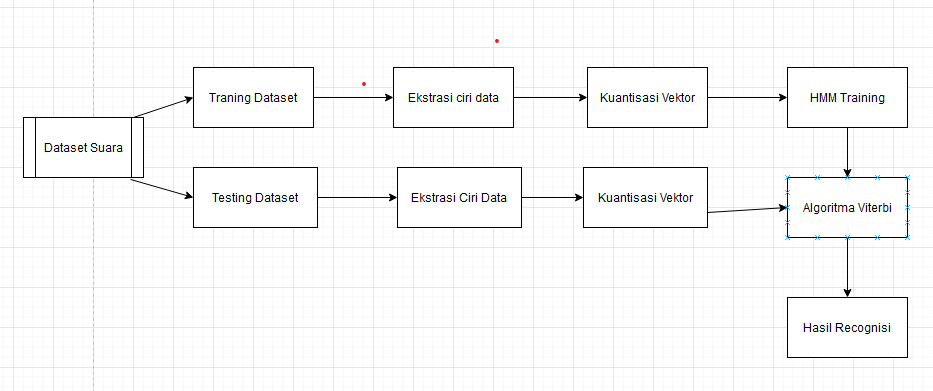
\includegraphics[width=4cm]{figures/1174096/tugas6/teori_1.PNG}
		\caption{Ilustrasi MFCC}
	\end{figure}

	\item Jelaskan konsep dasar neural network
	\hfill\break
    Neural Network merupakan kumpulan algoritma yang terinspirasi konsepnya dari otak manusia. Konsep tersebut diantaranya mempelajari pola - pola yang diberikan oleh inputan lain. Untuk menerima data, biasanya Neural Network mendapatkannya dari inputan sensor atau komputasi otomatis yang sudah disediakan oleh programmer untuk melakukan input otomatis ke media Neural Network. Data yang diterima berupa numerik yang terdapat pada vektor yang sesuai dengan data berwujud aslinya. Neural network mengkluster dan menklasifikasikan data untuk dapat disesuaikan dengan parameter - parameter yang sudah ada. 
	
    \begin{figure}[H]
	\centering
		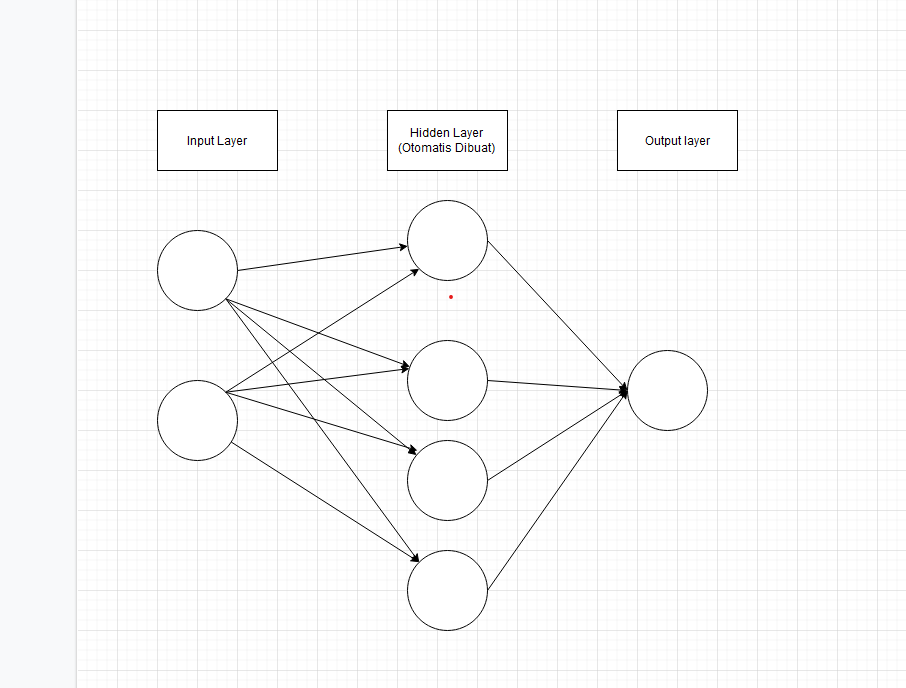
\includegraphics[width=4cm]{figures/1174096/tugas6/teori_2.PNG}
		\caption{konsep neural network}
	\end{figure}


	\item Jelaskan konsep pembobotan dalam neural network
	\hfill\break
	Pembobotan dalam neural network yaitu digunakan untuk membedakan objek inputan atau variabel inputan untuk AI misalkan apel dan jeruk digunakan untuk variabel inputan maka dibuat pembobotan anatara kedua benda tersebut untuk menentukan output yang pasti dari inputan yang dilakukan untuk lebih jelasnya dapat dilihat pada gambar.
    \begin{figure}[H]
	\centering
		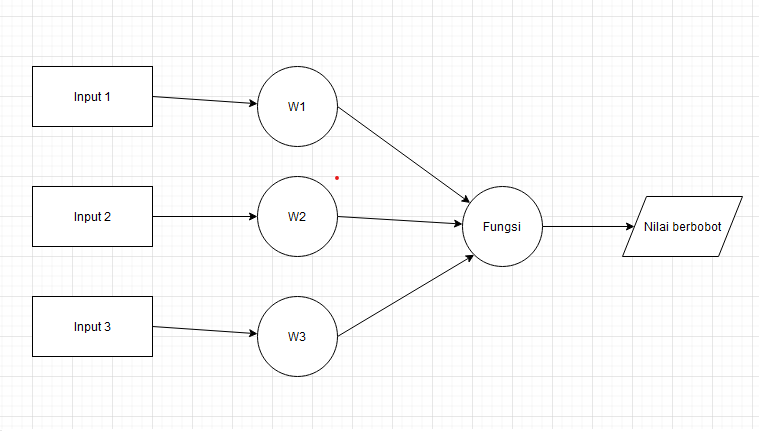
\includegraphics[width=4cm]{figures/1174096/tugas6/teori_3.PNG}
		\caption{pembobotan dalam neural network}
	\end{figure}

	\item Jelaskan konsep fungsi aktivasi dalam neural network.
	\hfill\break
	Fungsi aktivasi merupakan fungsi yang digunakan untuk mendapatkan output neuron dari nilai inputnya. Fungsi aktivasi akan melakukan penilaian jika output yang dikeluarkan telah mencapai hasil yang telah ditentukan. 
    \begin{figure}[H]
	\centering
		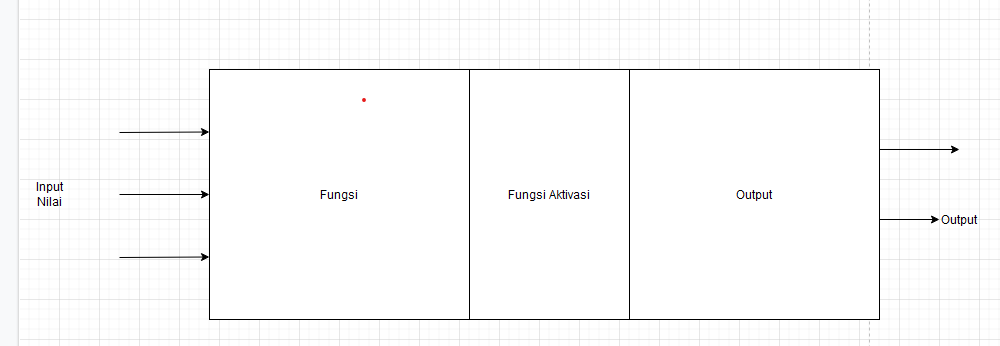
\includegraphics[width=4cm]{figures/1174096/tugas6/teori_4.PNG}
		\caption{aktivasi dalam neural network}
	\end{figure}

	\item Jelaskan cara membaca hasil plot dari MFCC,.
	\hfill\break
	Untuk membaca hasil plotting dari MFCC diantaranya menentukan terlebih dahulu batas minimal gelombang suara (Hz) dan batas maksimal dari suara tersebut. Lalu warna yang paling pekat merupakan hasil dari penglohana data tersebut. Saat membaca file, gelommbang akan diklasifikasikan dengan cara mengkalkulasikan jarak diantara vektor 12 Dimensi. 
	\begin{figure}[H]
	\centering
		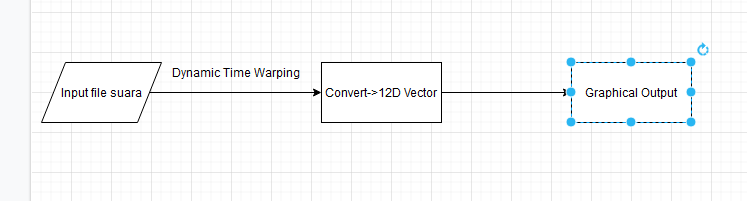
\includegraphics[width=4cm]{figures/1174096/tugas6/teori_5.PNG}
		\caption{Cara membaca hasil plot dari MFCC}
	\end{figure}

	\item Jelaskan apa itu one-hot encoding
	\hfill\break
	One-hot encoding merupakan numerisasi nilai untuk dapat mengindikasikan sebuah status. Karena butuhnya mesin untuk membaca nilai binary, biasanya mesin akan mengkonversi (Decode) terlebih dahulu untuk dapat membaca nilai. Namun saat nilai dilakukan Encoding dengan metode ini, maka nilai tidak perlu di encode lagi karena nilai yang ada sudah merupakan nilai binary. 
	\begin{figure}[H]
	    \centering
	    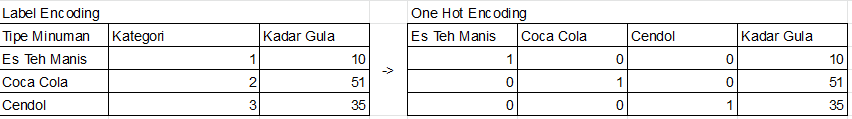
\includegraphics[width=4cm]{figures/1174096/tugas6/teori_6.PNG}
	    \caption{One hot encoding}
    \end{figure}

    \item Jelaskan apa fungsi dari np.unique dan to categorical dalam kode program
    \hfill\break
    Fungsi ini akan mengembalikan array dengan elemen yang berbeda - beda dalam input array. Fungsi ini akan memangkas nilai sehingga hanya beberapa nilai saja yang ada dan nilai tersebut harus berbeda dengan yang lainnya. Biasanya fungsi ini untuk mengidentifikasi jenis nilai atau nilai apa saja yang terdapat pada array yang bersangkutan. to categorical merupakan fungsi untuk mengkonversikan dataset menjadi sebuah beberapa kategori kelas yang ditentukan. Nilai itu sendiri akan diubah menjadi bentuk 'One-hot vector' untuk dapat dibaca oleh komputer.
    \lstinputlisting[firstline=8, lastline=17]{src/1174096/6/teori.py}
    \begin{figure}[H]
	    \centering
	    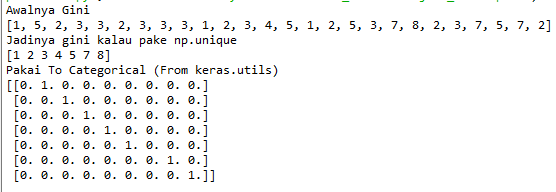
\includegraphics[width=4cm]{figures/1174096/tugas6/teori_7.PNG}
	    \caption{fungsi np.unique dan to categorial}
    \end{figure}

    \item Jelaskan apa fungsi dari Sequential dalam kode program
    \hfill\break
    Sequential berfungsi untuk mencari nilai yang dicari berdasarkan pencarian berurutan sesuai numeric terendah ke tertinggi atau sebaliknya. Sequential dapat digunakan dalam pencarian data vektor untuk mengetahui apakah nilai ada atau tidak. Karena vektor isinya berupa nilai numeric, maka pencarian sequential dapat dijadikan sebagai salah satu metode untuk mencari data tersebut.
    \lstinputlisting[firstline=20, lastline=25]{src/1174096/6/teori.py}
    \begin{figure}[H]
	    \centering
	    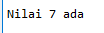
\includegraphics[width=4cm]{figures/1174096/tugas6/teori_8.PNG}
	    \caption{fungsi sequential}
    \end{figure}
\end{enumerate}

\subsection{Praktek Program}
\begin{enumerate}
	\item  Jelaskan isi dari data GTZAN Genre Collection dan data dari freesound. Buat kode program untuk meload data tersebut untuk digunakan pada MFCC. Jelaskan arti dari setiap baris kode yang dibuat
	\hfill\break
	\lstinputlisting[firstline=9, lastline=28]{src/1174096/6/praktek.py}
	Kode di atas menjelaskan isi data GTZAN. Ini adalah kumpulan data yang berisi 10 genre lagu dengan masing-masing genre memiliki 100 lagu yang akan kami lakukan proses MFCC dan juga freesound yang hanya berisi konten lagu, jika GTZAN memiliki beberapa genre jika freesound hanya untuk 1 lagu dan disini kita membuat fungsi untuk membaca file audio dan outputnya sebagai plot, hasilnya adalah sebagai berikut:
	\begin{figure}[H]
	\centering
		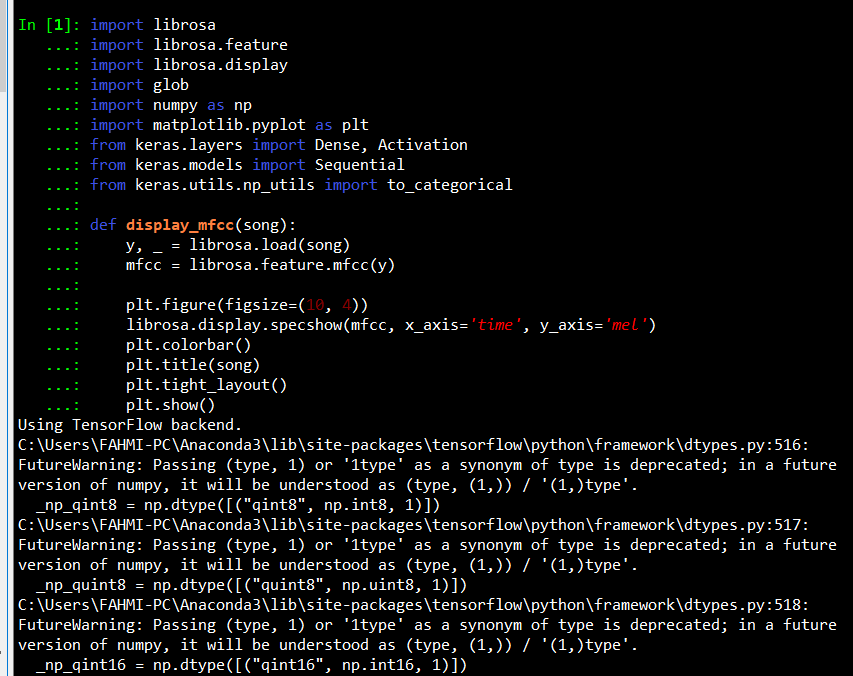
\includegraphics[width=4cm]{figures/1174096/tugas6/hasil1.PNG}
		\caption{Hasil Soal 1.}
	\end{figure}

	\item  Jelaskan perbaris kode program dengan kata-kata dan dilengkapi ilustrasi gambar fungsi dari display mfcc()
	\hfill\break
	\lstinputlisting[firstline=29, lastline=50]{src/1174096/6/praktek.py}
	Kode di atas akan menampilkan hasil dari proses mfcc yang sudah dibuat fungsi pada soal 1, yaitu display mfcc() dan akan menampilkan plot dari pembacaan file audio. Berikut adalah hasil setelah saya lakukan running dan pembacaan file audio :
	\begin{figure}[H]
	\centering
		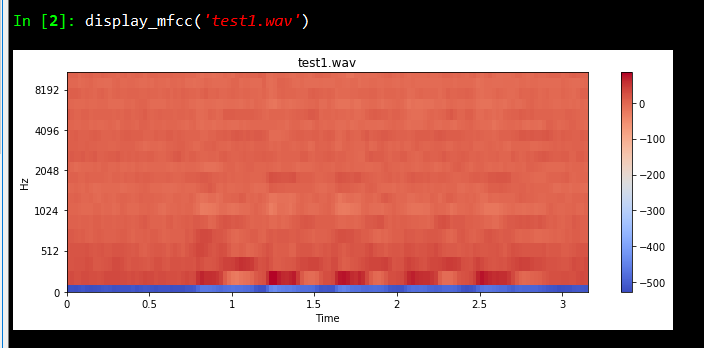
\includegraphics[width=4cm]{figures/1174096/tugas6/hasil2_1.PNG}
		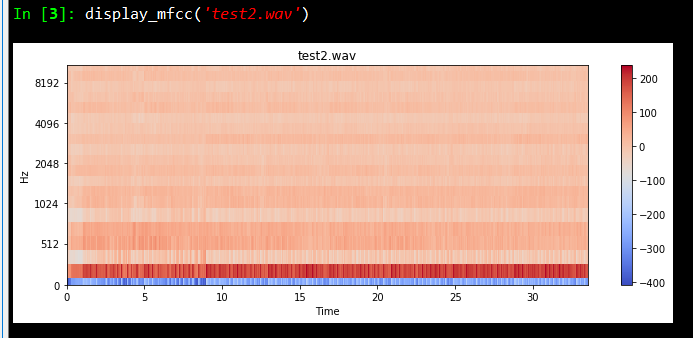
\includegraphics[width=4cm]{figures/1174096/tugas6/hasil2_2.PNG}
		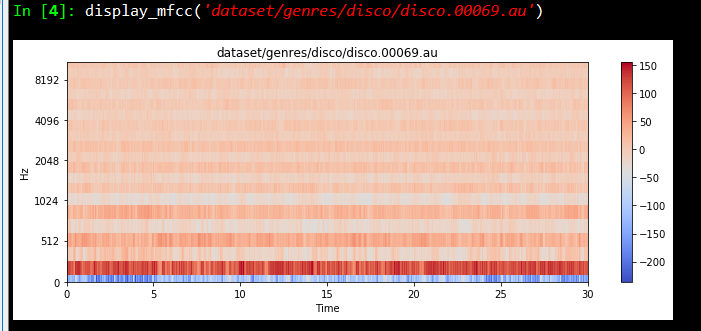
\includegraphics[width=4cm]{figures/1174096/tugas6/hasil2_3.PNG}
		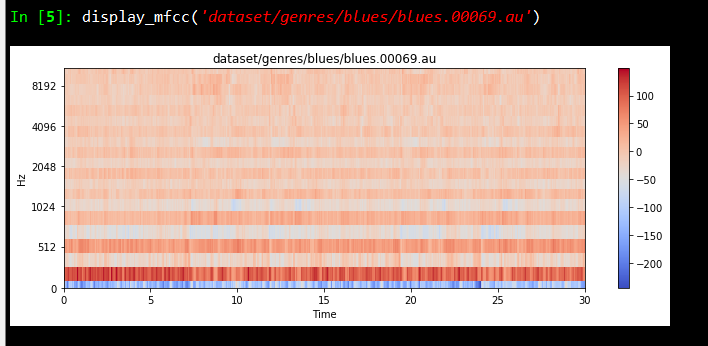
\includegraphics[width=4cm]{figures/1174096/tugas6/hasil2_4.PNG}
		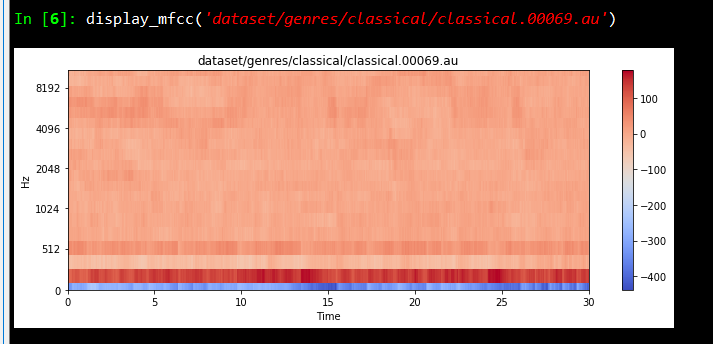
\includegraphics[width=4cm]{figures/1174096/tugas6/hasil2_5.PNG}
		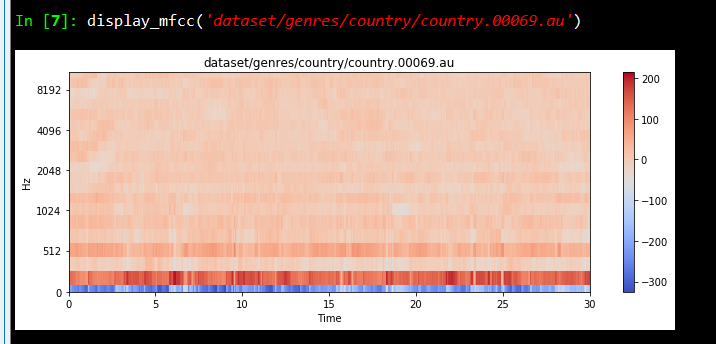
\includegraphics[width=4cm]{figures/1174096/tugas6/hasil2_6.PNG}
		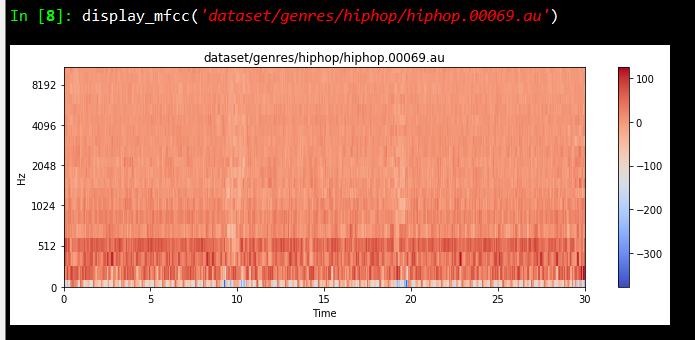
\includegraphics[width=4cm]{figures/1174096/tugas6/hasil2_7.PNG}
		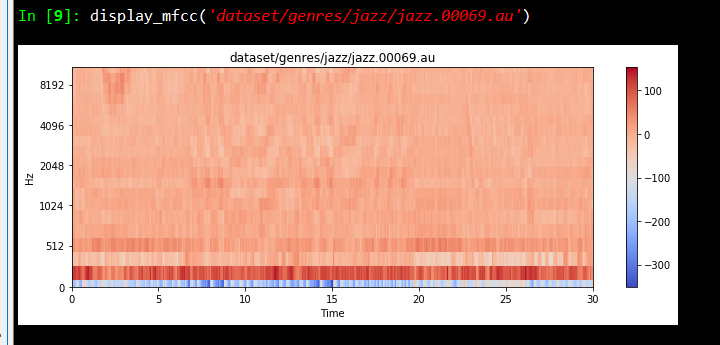
\includegraphics[width=4cm]{figures/1174096/tugas6/hasil2_8.PNG}
		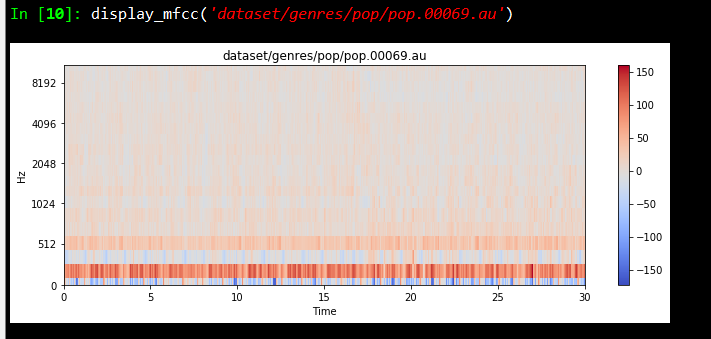
\includegraphics[width=4cm]{figures/1174096/tugas6/hasil2_9.PNG}
		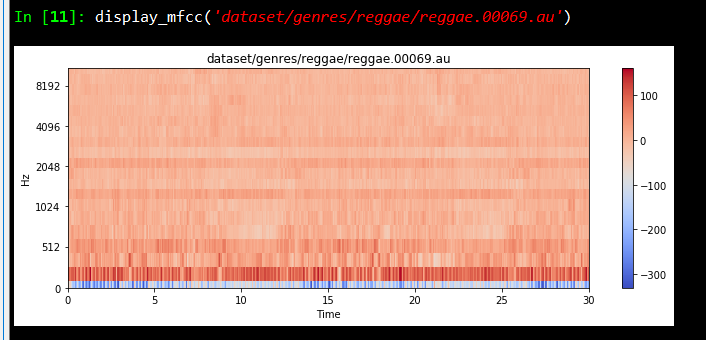
\includegraphics[width=4cm]{figures/1174096/tugas6/hasil2_10.PNG}
		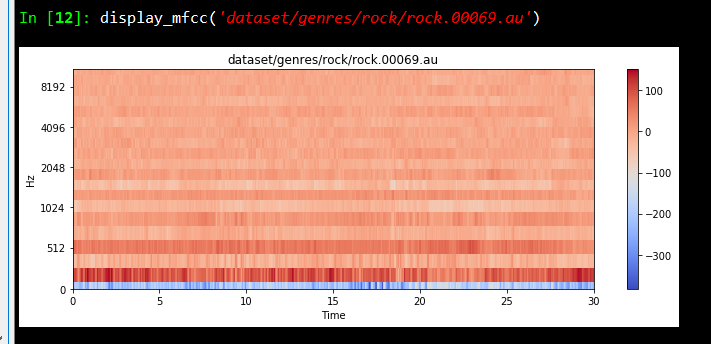
\includegraphics[width=4cm]{figures/1174096/tugas6/hasil2_11.PNG}
		\caption{Hasil Soal 2.}
	\end{figure}

	\item Jelaskan perbaris kode program dengan kata-kata dan dilengkapi ilustrasi gambar fungsi dari extract features song(). Jelaskan juga mengapa yang diambil 25.000 baris pertama?
	\hfill\break
	\lstinputlisting[firstline=53, lastline=61]{src/1174096/6/praktek.py}
	Baris pertama itu untuk membuat fungsi extract\_features\_song(f). Pada baris kedua itu akan me-load data inputan dengan menggunakan librosa. Lalu selanjutnya untuk membuat sebuah fitur untuk mfcc dari y atau parameter inputan. Lalu akan me-return menjadi array dan akan mengambil 25000 data saja dari hasil vektorisasi dalam 1 lagu. Hasilnya adalah sebagai berikut :
	\begin{figure}[H]
	\centering
		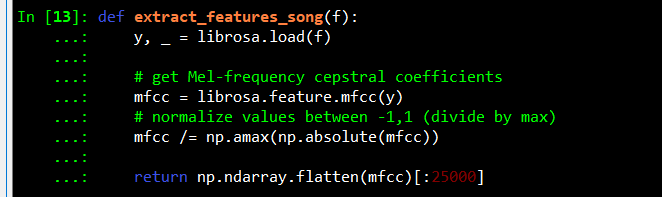
\includegraphics[width=4cm]{figures/1174096/tugas6/hasil3.PNG}
		\caption{Hasil Soal 3.}
	\end{figure}

	\item Jelaskan perbaris kode program dengan kata-kata dan dilengkapi ilustrasi gambar fungsi dari generate features and labels().
	\hfill\break
	\lstinputlisting[firstline=65, lastline=82]{src/1174096/6/praktek.py}
	Kode di atas dapat digunakan untuk melakukan fungsi yang sebelumnya telah kita lakukan. Kemudian di bagian genre yang disesuaikan dengan dataset nama folder. Untuk baris berikutnya akan mengulang genre folder dengan ekstensi .au. Maka itu akan memanggil fungsi ekstrak lagu. Setiap file dalam folder itu akan diekstraksi menjadi vektor dan akan ditambahkan ke fitur. Dan fungsi yang ditambahkan adalah untuk menumpuk file yang telah di-vektor-kan. Hasil kode tidak menampilkan output. Hasilnya adalah sebagai berikut :
	\begin{figure}[H]
	\centering
		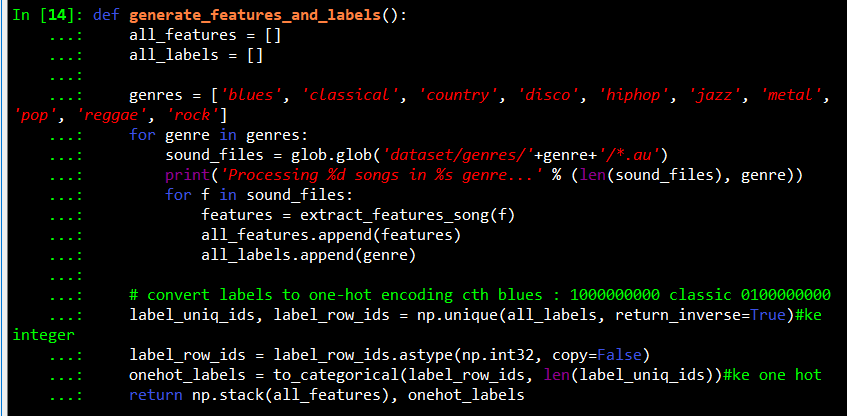
\includegraphics[width=4cm]{figures/1174096/tugas6/hasil4.PNG}
		\caption{Hasil Soal 4.}
	\end{figure}

	\item Jelaskan dengan kata dan praktek kenapa penggunaan fungsi generate features and labels() sangat lama ketika meload dataset genre. 
	\hfill\break
	\lstinputlisting[firstline=86, lastline=89]{src/1174096/6/praktek.py}
	Kode diatas berfungsi untuk melakukan load variabel features dan labels. Mengapa memakan waktu yang lama ? Karena mesin akan melakukan vektorisasi terhadap semua file yang berada pada setiap foldernya, di sini terdapat 10 folder dengan masing-masing folder terdiri atas 100 buah lagu, setiap lagu tersebut akan dilakukan vektorisasi atau ekstraksi data menggunakan mfcc. Oleh karena itu, proses cukup memakan waktu. Hasilnya adalah sebagai berikut :
	\begin{figure}[H]
	\centering
		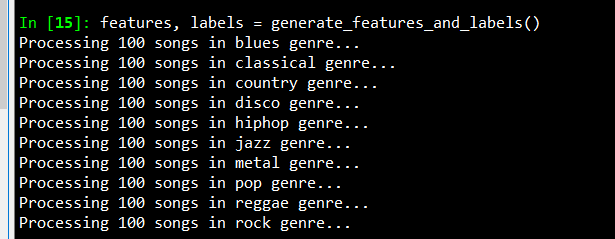
\includegraphics[width=4cm]{figures/1174096/tugas6/hasil5_1.PNG}
		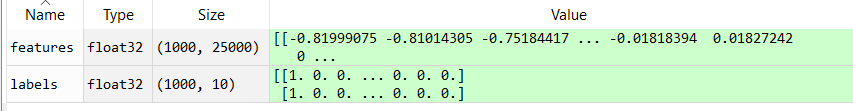
\includegraphics[width=4cm]{figures/1174096/tugas6/hasil5_2.PNG}
		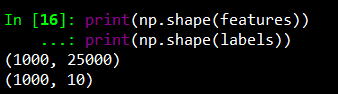
\includegraphics[width=4cm]{figures/1174096/tugas6/hasil5_3.PNG}
		\caption{Hasil Soal 5.}
	\end{figure}

	\item Jelaskan kenapa harus dilakukan pemisahan data training dan data set sebesar 80 persen? 
	\hfill\break
	\lstinputlisting[firstline=91, lastline=109]{src/1174096/6/praktek.py}
	Kode diatas berfungsi untuk melakukan training split 80\%. Karena supaya mesin dapat terus belajar tentang data baru, jadi ketika prediksi dibuat tentang data yang terlatih itu bisa mendapatkan persentase yang cukup bagus. Hasilnya adalah sebagai berikut :
	\begin{figure}[H]
	\centering
		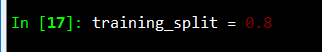
\includegraphics[width=4cm]{figures/1174096/tugas6/hasil6_1.PNG}
		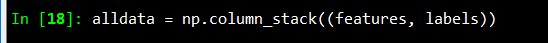
\includegraphics[width=4cm]{figures/1174096/tugas6/hasil6_2.PNG}
		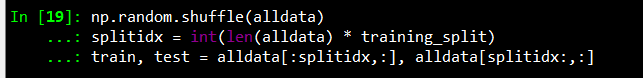
\includegraphics[width=4cm]{figures/1174096/tugas6/hasil6_3.PNG}
		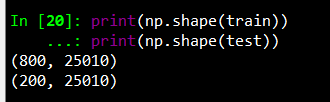
\includegraphics[width=4cm]{figures/1174096/tugas6/hasil6_4.PNG}
		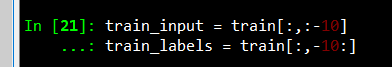
\includegraphics[width=4cm]{figures/1174096/tugas6/hasil6_5.PNG}
		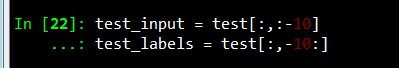
\includegraphics[width=4cm]{figures/1174096/tugas6/hasil6_6.PNG}
		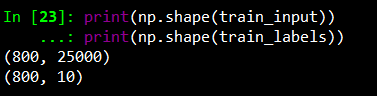
\includegraphics[width=4cm]{figures/1174096/tugas6/hasil6_7.PNG}
		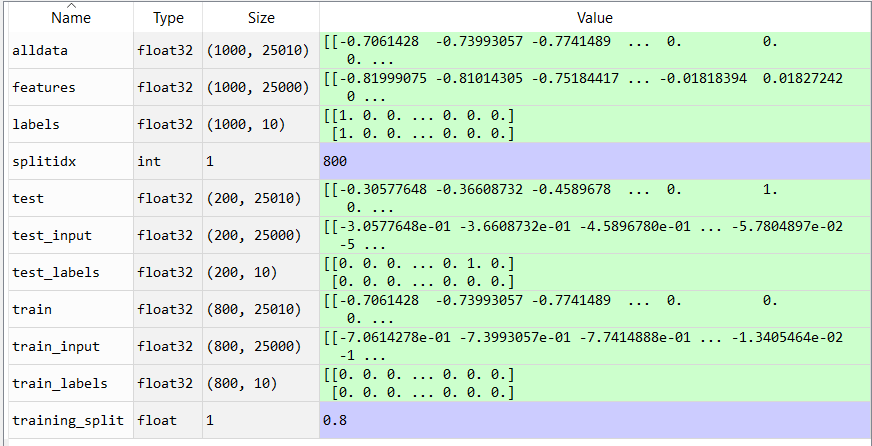
\includegraphics[width=4cm]{figures/1174096/tugas6/hasil6_8.PNG}
		\caption{Hasil Soal 6.}
	\end{figure}

	\item Praktekkan dan jelaskan masing-masing parameter dari fungsi Sequential().
	\hfill\break
	\lstinputlisting[firstline=112, lastline=117]{src/1174096/6/praktek.py}
	fungsi Sequential() ialah Sebuah model untuk menentukan izin pada setiap neuron, di sini adalah 100 dense yang merupakan 100 neuron pertama dari data pelatihan. Fungsi dari relay itu sendiri adalah untuk mengaktifkan neuron atau input yang memiliki nilai maksimum. Sedangkan untuk dense 10 itu adalah output dari hasil neuron yang telah berhasil diaktifkan, untuk dense 10 diaktifkan menggunakan softmax. Hasilnya adalah sebagai berikut :
	\begin{figure}[H]
	\centering
		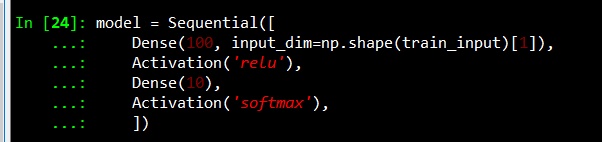
\includegraphics[width=4cm]{figures/1174096/tugas6/hasil7.PNG}
		\caption{Hasil Soal 7.}
	\end{figure}

	\item Praktekkan dan jelaskan masing-masing parameter dari fungsi compile().
	\hfill\break
	\lstinputlisting[firstline=119, lastline=122]{src/1174096/6/praktek.py}
	Model Compile di perjelas dengan gambar dibawah, Hasil output pada kode tersebut seperti gambar  menjelaskan bahwa dense pertama itu memiliki 100 neurons dengan parameter sekitar 2 juta lebih dengan aktviasi 100, jadi untuk setiap neurons memiliki masing-masing 1 aktivasi. Sama halnya seperti dense 2 memiliki jumlah neurons sebanyak 10 dengan parameter 1010 dan jumlah aktivasinya 10 untuk setiap neurons tersebut dan total parameternya sekitar 2.5 juta data yang akan dilatih pada mesin tersebut.
	\begin{figure}[H]
	\centering
		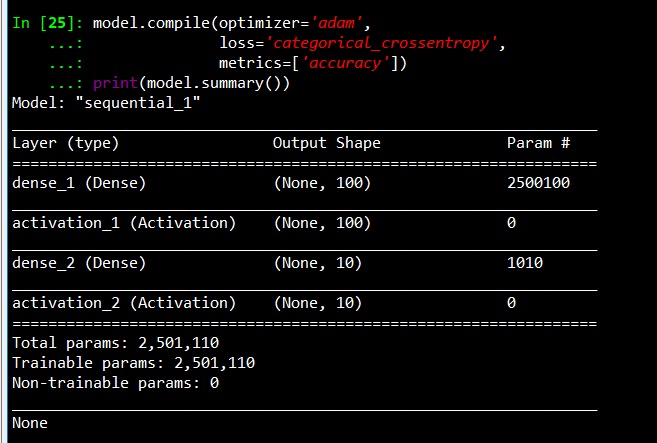
\includegraphics[width=4cm]{figures/1174096/tugas6/hasil8.PNG}
		\caption{Hasil Soal 8.}
	\end{figure}

	\item Praktekkan dan jelaskan masing-masing parameter dari fungsi fit().
	\hfill\break
	\lstinputlisting[firstline=124, lastline=125]{src/1174096/6/praktek.py}
	Kode tersebut berfungsi untuk melatih mesin dengan data training input dan training label. Epochs ini merupakan iterasi atau pengulangan berapa kali data tersebut akan dilakukan. Batch\_size ini adalah jumlah file yang akan dilakukan pelatihan pada setiap 1 kali pengulangan. Sedangkan validation\_split itu untuk menentukan presentase dari cross validation atau k-fold sebanyak 20\% dari masing-masing data pengulangan, hasilnya adalah sebagai berikut :
	\begin{figure}[H]
	\centering
		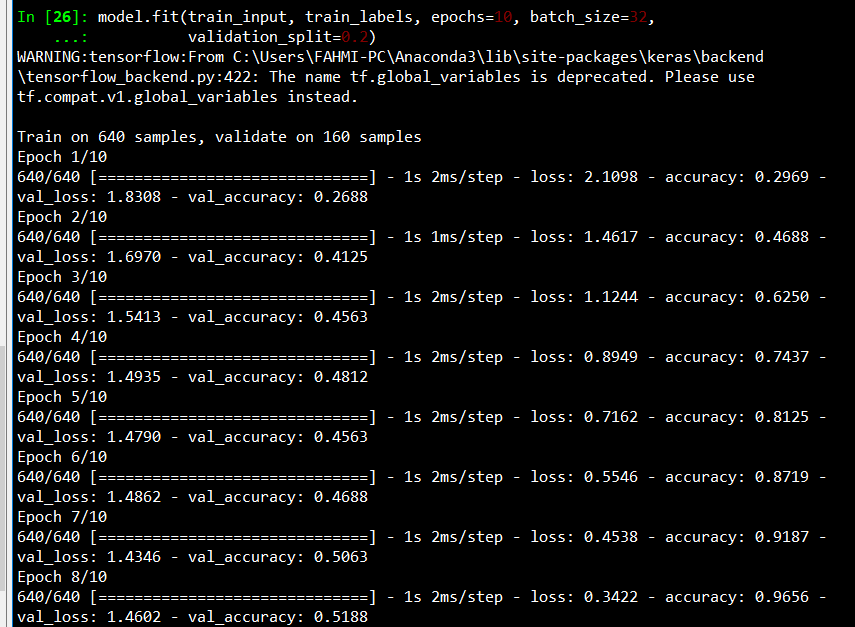
\includegraphics[width=4cm]{figures/1174096/tugas6/hasil9.PNG}
		\caption{Hasil Soal 9.}
	\end{figure}

	\item Praktekkan dan jelaskan masing-masing parameter dari fungsi evaluate()
	\hfill\break
	\lstinputlisting[firstline=127, lastline=130]{src/1174096/6/praktek.py}
	Fungsi evaluate atau evaluasi ini ialah untuk menguji data pengujian setiap file. Di sini ada prediksi yang hilang, artinya mesin memprediksi data, sedangkan untuk keseluruhan perjanjian sekitar 55\%, hasilnya adalah sebagai berikut :
	\begin{figure}[H]
	\centering
		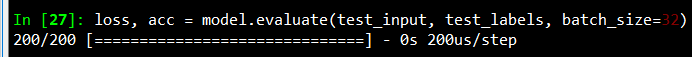
\includegraphics[width=4cm]{figures/1174096/tugas6/hasil10_1.PNG}
		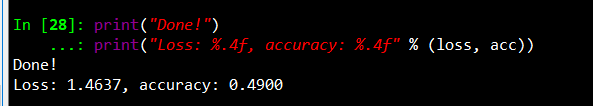
\includegraphics[width=4cm]{figures/1174096/tugas6/hasil10_2.PNG}
		\caption{Hasil Soal 10.}
	\end{figure}

	\item Praktekkan dan jelaskan masing-masing parameter dari fungsi predict().
	\hfill\break
	\lstinputlisting[firstline=133, lastline=133]{src/1174096/6/praktek.py}
	Fungsi Predict ialah untuk menghasilkan suatu nilai yang sudah di prediksi dari data training sebelumnya. Gambar dibawah ini menjelaskan file yang di jalankan tersebut termasuk ke dalam genre apa, hasilnya bisa dilihat pada gambar tersebut presentase yang paling besar yakni genre rock. Maka lagu tersebut termasuk ke dalam genre rock dengan perbandingan presentase hasil prediksi.
	\begin{figure}[H]
	\centering
		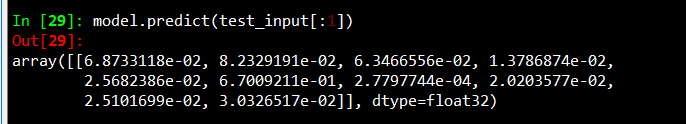
\includegraphics[width=4cm]{figures/1174096/tugas6/hasil11.PNG}
		\caption{Hasil Soal 11.}
	\end{figure}
\end{enumerate}

\subsection{Penanganan Error}
\begin{enumerate}
	\item NameError : name is not defined
	\begin{figure}[H]
		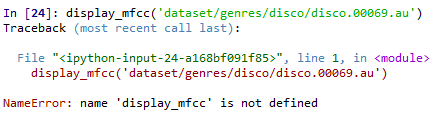
\includegraphics[width=4cm]{figures/1174096/tugas6/error.PNG}
		\centering
		\caption{NameError}
	\end{figure}
	\item Tuliskan Kode Error dan Jenis Error
	\begin{itemize}
		\item NameError
	\end{itemize}
	\item Cara Penangan Error
	\begin{itemize}
		\item NameError
		\hfill\break
		Error terjadi karena nama fungsi belum didefenisikan. Cara mengatasinya yaitu dengan mendeefenisikan terlebih dahulu nama fungsi pada baris kode diatasnya sebelum melakukan pemanggilan fungsi
	\end{itemize}
\end{enumerate}

\subsection{Bukti Tidak Plagiat}
\begin{figure}[H]
\centering
	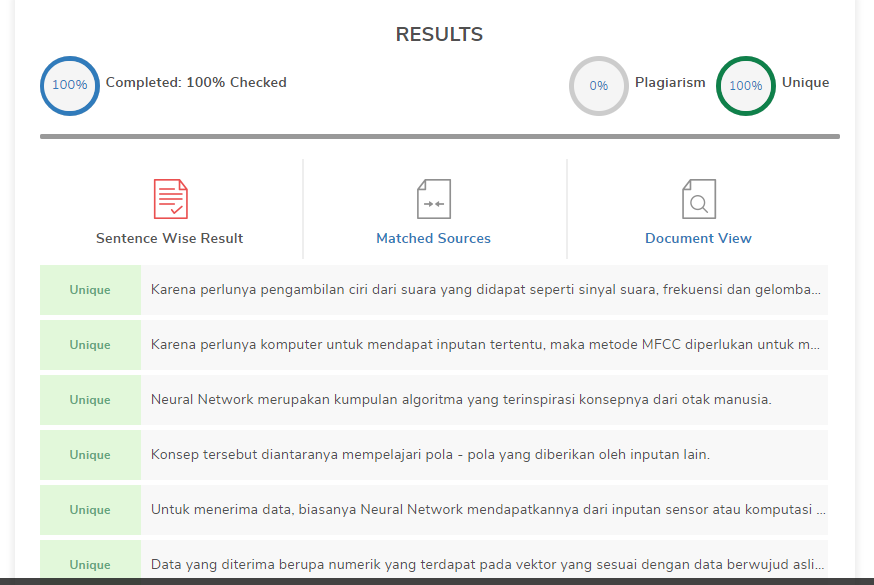
\includegraphics[width=4cm]{figures/1174096/tugas6/Plagiarisme.PNG}
	\caption{Bukti Tidak Melakukan Plagiat Chapter 6}
\end{figure}
